\documentclass[14pt,oneside]{article}
\usepackage[utf8]{inputenc}  
\usepackage[T1]{fontenc}
\usepackage{amsmath,amssymb,bm}
\usepackage{titlesec}
\usepackage{titletoc}
\usepackage{graphicx}
\usepackage[margin=2.5cm]{geometry}
\usepackage[french]{babel}
\usepackage{hyperref}
\hypersetup {colorlinks=true,linkcolor=blue,urlcolor=blue}
\AddThinSpaceBeforeFootnotes
\FrenchFootnotes
\usepackage{ae,lmodern}
\usepackage{sectsty}
\usepackage[usenames,dvipsnames]{xcolor}
\usepackage{enumitem}
\usepackage{caption}
\usepackage{multicol}
\usepackage{pifont}
\usepackage{fancyhdr}
\pagestyle{fancy}
\rhead{Rapport}
\lhead{\leftmark}
\rfoot{Page \thepage}
\renewcommand{\headrulewidth}{2pt}
\renewcommand{\footrulewidth}{1pt}
\definecolor{Rapport}{RGB}{213,25,50}
\definecolor{airforceblue}{rgb}{0.36, 0.54, 0.66}
\definecolor{amber}{rgb}{1.0, 0.75, 0.0}
\sectionfont{\bfseries\color{Plum}\LARGE}
\subsectionfont{\color{Mulberry}}
\parskip=10pt
\setlength{\parindent}{1cm}
\begin{document}
\begin{titlepage}
\phantom{aaaaaaaaaaaaaaaaaaaaaaaaaaaaaaaaaaaaaaa
ytrfdytfugvghikuhjbiujbhaaaaaaaaaaaaaaa}


\begin{minipage}[c]{.46\linewidth}
		\centering
		
\includegraphics[scale=0.1]{logo} 
	\end{minipage}
\hfill%
\begin{minipage}[c]{.46\linewidth}
		\centering
		
\includegraphics[scale=0.04]{LE2P} 
\end{minipage}



\phantom{aaaaaaaaaaaaaaaaaaaaaaaaaaaaaaaaaaaaaaa
ytrfdytfugvghikuhjbiujbhaaaaaaaaaaaaaaa}
\center
\fbox{\begin{minipage}[t][1cm][c]{8cm}
\begin{center}
{\huge \bfseries \textcolor{Rapport}{Feuille de Route}}
\end{center}
\end{minipage}}\\[0.5cm]
\textbf{\Large \color{Mulberry} .}\\[0.5cm] 
\begin{minipage}{0.5\textwidth}
\begin{flushleft} \large
\hspace{0.22\textwidth}\emph{\underline{Auteurs}:}\\
\begin{multicols}{2}
\begin{itemize}[font=\color{airforceblue} \Large, label=\ding{47}, leftmargin=0cm]
\item{Hermanda \textsc{Tandrayen} \\ {\small{35008782}}}
\item{Sanjy \textsc{Maksim} \\ {\small{35001087}}}
\end{itemize}
\end{multicols}
\end{flushleft}
\end{minipage}
\begin{minipage}{0.45\textwidth}
\begin{flushright} \large
\emph{\underline{Encadrants}:}\phantom{aaaaa}\\

\begin{itemize}[font=\color{amber} \Large, label=\ding{80}, leftmargin=3.5cm]
\item{Beatrice \textsc{Morel}}
\item{Alexandre \textsc{Graillet}}
\item{Mathieu \textsc{Delsaut}}
\end{itemize}

\end{flushright}
\end{minipage}\\[0cm]
\vspace{2 cm}
\begin{center}
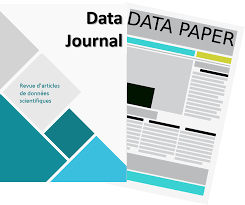
\includegraphics[scale=1]{1.png} 
\end{center}
\vspace{1cm}

\begin{center}
2019/2020
\end{center}
\vfill
\end{titlepage}


\newpage
\part*{Objectifs de la semaine}
\begin{itemize}
	\item Faire des recherches sur la FAIR
\end{itemize}

\part*{Taches effectuées}
\section*{Recherche sur le principe de "FAIR"}

\noindent FAIR est un acronyme pour:
\begin{itemize}
    \item F = findable (trouvables),
    \item A = accessible (accessibles),
    \item I = interoperable (interopérables),
    \item R = reusable (réutilisables),
\end{itemize}

\phantom{czd}\\

\noindent POUR ÊTRE TROUVABLES:
    \begin{itemize}
    \item Les (méta) données se voient attribuer un identifiant globalement unique et éternellement persistant.
    \item les données sont décrites avec des métadonnées riches.
    \item Les (méta) données sont  enregistrées ou indexées dans une ressource interrogeable.
    \item les métadonnées  spécifient  l'identificateur de données.
    \end{itemize}

\phantom{czd}\\

\noindent POUR ÊTRE ACCESSIBLES:
    \begin{itemize}
    \item Les données (méta) sont récupérables grâce à leur identifiant à l' aide d'  un protocole de communication normalisé.
    \item Le protocole est ouvert, libre et universellement applicable.
    \item Le protocole permet une procédure d'authentification et d'autorisation, le cas échéant.
    \item Les métadonnées sont accessibles , même lorsque les données ne sont plus disponibles.
    \end{itemize}


phantom{czd}\\

\noindent POUR ÊTRE INTEROPÉRABLES:
    \begin{itemize}
    \item Les (méta) données utilisent un langage formel, accessible, partagé et largement applicable pour la représentation des connaissances.
    \item  Les vocabulaires d' utilisation (méta) de données  qui suivent les principes de FAIR.
    \item Les (méta) données incluent  des références qualifiées  à d'autres (méta) données.
    \item Les métadonnées sont accessibles , même lorsque les données ne sont plus disponibles.
    \end{itemize}

\newpage

\noindent POUR ÊTRE RÉUTILISABLES:
    \begin{itemize}
    \item Les méta (données) ont une pluralité d'attributs précis et pertinents.
    \item Les (méta) données sont publiées avec une licence d'utilisation des données claire et accessible.
    \item Les (méta) données sont associées à leur  provenance.
    \item Les (méta) données  répondent aux normes de la communauté applicables au domaine.
    \end{itemize}
Texte extrait du site GO FAIR: \url{https://www.go-fair.org/fair-principles/}

\section*{Open acces et FAIR, c'est quoi la différence ?}

Des données ouvertes sans restriction (téléchargeables librement et gratuitement, licence imposant le minimum de contrainte, etc) sont 100\% accessible.\\
Mais des données scientifiques peuvent aussi être FAIR tout en étant en accès restreint, ou sous embargo, si cela se justifie. Dans ce cas il faut au minimum que les métadonnées soient elles mêmes accessibles.

- éxtrait de texte du livre\\
\underline{Cloudy, increasingly FAIR; revisiting the FAIR Data guiding principles for the European Open Science Cloud}\\
\phantom{CA}\\
Nous pouvons etre un peut plus éclairé sur le sujet:\\
\phantom{CA}\\
« FAIR n’est pas égal à Open : « A » dans FAIR signifie « Accessible dans des conditions bien définies ». Il peut y avoir des raisons légitimes de protéger l’accès public aux données et aux services générés par le financement public. Cela comprend la protection de la vie privée, la sécurité nationale et la compétitivité. Les principes de FAIR, bien qu’inspirés par la science ouverte, ne traitent pas explicitement et délibérément des questions morales et éthiques relatives à l’ouverture des données. Dans l’Internet envisagé de FAIR Data and Services, la mesure dans laquelle une donnée est disponible, ou même annoncée comme étant disponible (via ses métadonnées) est entièrement à la discrétion du propriétaire des données. FAIR ne parle que de la nécessité de décrire un processus – mécanisé ou manuel – pour accéder aux données découvertes ; l’obligation de décrire ouvertement et abondamment le contexte dans lequel ces données ont été produites, afin de permettre l’évaluation de leur utilité; de définir explicitement les conditions dans lesquelles elles peuvent être réutilisées; et fournir des instructions claires sur la façon de les citer lorsqu’ils sont réutilisés » \\
\phantom{czc}\\
Doi de l'article: \url{https://doi.org/10.3233/ISU-170824 }
\newpage
\part*{Objectifs pour la semaine prochaine}
\begin{itemize}
	\item Recherche questions pertinentes sur DMP
\end{itemize}


\end{document}
